\documentclass{article}

\usepackage[paper=a4paper,margin=0.9in]{geometry}

\usepackage{mathtools}
\usepackage{enumitem} % enumeration label options
\usepackage{amsfonts} % \mathbb
\usepackage{mathrsfs} % \mathscr
\usepackage{amsthm}
\usepackage{tikz-cd}

\setlength{\parindent}{0pt}

\newtheorem*{conjecture}{Conjecture}
\newtheorem*{theorem}{Theorem}
\newtheorem*{corollary}{Corollary}
\newtheorem*{lemma}{Lemma}

\theoremstyle{definition}
\newtheorem*{definition}{Definition}
\newtheorem*{example}{Example}
\newtheorem*{remark}{Remark}
\newtheorem*{exercise}{Exercise}

\DeclareMathOperator{\Bl}{Bl}
\DeclareMathOperator{\Spec}{Spec}
\DeclareMathOperator{\exc}{exc}
\DeclareMathOperator{\supp}{supp}
\DeclareMathOperator{\cosupp}{cosupp}

\newcommand{\sm}{\mathrm{sm}}

\newcommand{\I}{\mathscr{I}}
\newcommand{\J}{\mathscr{J}}
\renewcommand{\O}{\mathcal{O}}
\newcommand{\A}{\mathbb{A}}
\renewcommand{\P}{\mathbb{P}}
\newcommand{\N}{\mathbb{N}}
\newcommand{\Z}{\mathbb{Z}}
\newcommand{\Q}{\mathbb{Q}}
\newcommand{\R}{\mathbb{R}}
\newcommand{\C}{\mathbb{C}}

\title{Notes for ``Birational Geometry'' by Calum Spicer}
\author{Calum Crossley}
\date{LTCC 2023-2024}

\begin{document}

\maketitle

\section*{Overview}

The course will assume the content of Hartshorne\footnote{With the caveat that
he doesn't remember what exactly is and isn't in Hartshorne.}. We will look at
two main topics which may initially not look hugely related to birational
geometry, but in fact encompass a lot of the important ideas.
\begin{itemize}
    \item Moduli spaces: These are schemes / algebraic spaces / stacks / e.t.c.
        associated to a collection of algebraic objects (e.g. curves, surfaces,
        sheaves, ...).

    \item Foliations: These are a clever way of decomposing a space into
        subspaces, or analogously considering fibres in a fibre space.
\end{itemize}

\section*{Singularities and Adjunction}

All schemes are considered over a field $k$ of characteristic 0.

\begin{example}
    Consider $\A^2\cong\Spec k[x,y,t]/(xy-t)\xrightarrow{f}\Spec k[t]=\A^1$. For
    points $p\ne0$ in $\A^1$, the fibre $f^{-1}(p)$ is a smooth curve (a conic).
    For $p=0$ however  $f^{-1}(p)=V(xy)$ is a nodal singular curve. What does
    this say about the moduli space of curves? It says the moduli space of
    smooth curves is not proper / compact. (One might ask: why care about
    compactness for moduli spaces?)
\end{example}

\begin{exercise}
    Show that there does not exist an exact sequence
    \begin{equation*}
        0 \to \O(a) \to \Omega^1_{\P^2} \to \O(b) \to 0
    \end{equation*}
    of sheaves on $\P^2$ for any $a,b\in\Z$. As a consequence, there are no
    smooth foliations on $\P^2$.
\end{exercise}

So from looking at the simplest cases of our main topics: the moduli space of
curves, and foliations of $\P^2$, we see that singularities naturally arise.

\begin{theorem}[Hironaka]
    Let $X$ be a smooth variety over $k$ a field of characteristic 0, and let
    $\I\subseteq\O_X$ be an ideal sheaf. Then there exists a composition
    $b:X'\to X$ of blowups in smooth centres (i.e. along subvarieties which are
    smooth) contained in the singular locus of $X$, such that the cosupport of
    $b^{-1}\I=\I\cdot\O_X$ is a simple normal crossings divisor.
\end{theorem}

\begin{remark}
    The cosupport of an ideal sheaf is the support of the quotient;
    $\cosupp(\J)\coloneq\supp(\O_X/\J)$.
\end{remark}

\begin{corollary}[Resolution of Singularities]
    Let $X$ be a normal variety over $k$ a field of characteristic 0. Then there
    exists a composition $b:X'\to X$ of blowups in smooth centres contained in
    the singular locus of $X$, such that $X'$ is smooth and the exceptional
    locus $\exc(b)$ is a simple normal crossings divisor. As a consequence,
    every variety is birational to a smooth variety.
\end{corollary}

\begin{proof}
    Embed $X\hookrightarrow Y$ with $Y$ smooth, which is possible by Chow's
    lemma. Let $\pi:Y'\to Y$ be the composition of blowups obtained from
    Hironaka's lemma applied to the subvariety $X$. Then $\pi^{-1}(X)$ is a
    divisor, so at some point we must have blown up $X$. (Since we may assume
    $X$ has codimension at least 2 in $Y$.) Since we only blow up in smooth
    centres, at some point $X$ must have become smooth.
\end{proof}

The philosophy of Grothendieck is that we should study morphisms (of schemes
e.t.c.), not just the objects (schemes e.t.c.) themselves. Hironaka's theorem
tells us that we can make any morphism $X\to\Spec k$ smooth by blowing up. What
about general morphisms $f:X\to Z$?\footnote{We call a morphism smooth if it is
flat and has regular fibres.} The answer is no. Consider the example from above:
\begin{equation*}
    \A^2 \cong \Spec\frac{k[x,y,t]}{(xy-t)} \to \Spec k[t] = \A^1.
\end{equation*}
This morphism has a singularity at $(0,0)$ in $\A^2$ from the singular fibre
$V(xy)$ over $0\in\A^1$. If we blowup the origin the fibre over $0\in\A^1$
remains singular because of the exceptional divisor:
\begin{center}
    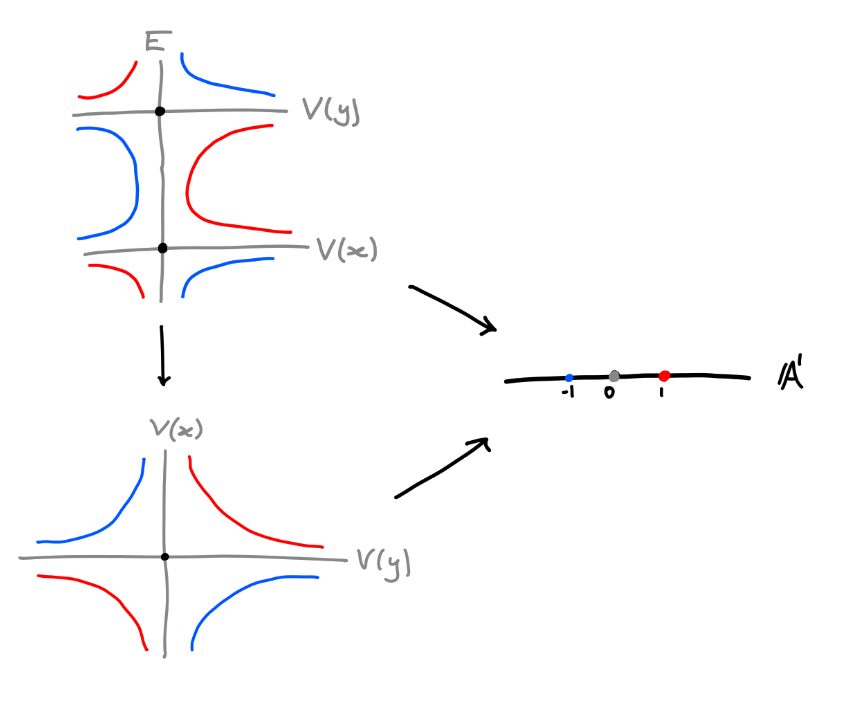
\includegraphics[scale=0.4]{hyperbola_blowup}
\end{center}
So the question becomes: what ``nice'' singularities should we allow?

\begin{definition}
    Let $f:(p,X)\to(q,Z)$ be a morphism of germs of smooth varieties. (Think of
    the germs as $\Spec\O_{X,p}$, or other possibilities.) We say $f$ is
    \emph{toroidal} if there exist \'Etale / analytic / formal coordinates
    $x_1,\ldots,x_n$ and $z_1,\ldots,z_k$ such that $f$ can be written as
    \begin{equation*}
        z_{i_l} = x_1^{m_{1,i_l}}\cdots x_n^{m_{n,i_l}}
    \end{equation*}
    for some collection of indices $i_l\in\{1,\ldots,k\}$. In other words, if
    $f$ can be written as monomials. We say a morphism $f:X\to Z$ is toroidal if
    all its germs are toroidal.
\end{definition}

\begin{example}
    Smooth morphisms are toroidal, by the inverse function theorem. The map
    $\Spec k[x,y,t]/(xy-t)\to\Spec k[t]$ is toroidal, as it can be written in
    coordinates as $(u,v)\mapsto uv$.
\end{example}

\begin{remark}
    Toroidal means formally locally isomorphic to a morphism of toric varieties.
    A good short reference for toric varieties is Fulton's book ``Introduction
    to Toric Varieties''.
\end{remark}

\begin{conjecture}
    Let $f:X\to Z$ be a morphism of varieties. Then there exists a diagram
    \begin{equation*}
        \begin{tikzcd}
            &X' \ar[r,"\beta"] \ar[d,"f'"] &X \ar[d,"f"] \\
            &Z' \ar[r,"\alpha"] &Z
        \end{tikzcd}
    \end{equation*}
    such that $\alpha$ and $\beta$ are birational maps and $f'$ is toroidal.
\end{conjecture}

\begin{remark}
    We are not assuming that $f$ has connected fibres here. (Recall connected
    fibres is equivalent to $f_*\O_X=\O_Z$ by Zariski's main theorem.) This is a
    naive way of generalizing Hironaka's theorem to morphisms, taking the
    ``nice'' class of singularities to be the toroidal singularities.
\end{remark}

\begin{theorem}[Abramovich--Karu]
    The above conjecture holds if $f:X\to Z$ is projective and has connected
    fibres (i.e. $f_*\O_X=\O_Z$).
\end{theorem}

\begin{definition}
    We say $f:X\to Z$ is \emph{semi-stable} if $f$ is toroidal and the
    scheme-theoretic fibres of $f$ are reduced.
\end{definition}

\begin{example}
    We cannot always achieve semi-stability by blowups; consider again the above
    example:
    \begin{align*}
        g : \Bl_{(0,0)}\A^2 \xrightarrow{b} \A^2 &\xrightarrow{f} \A^1 \\
            (x,y) &\mapsto xy
    \end{align*}
    This is a toroidal morphism, but we have
    \begin{align*}
        g^*(0)
            &= b^*(V(xy)) \\
            &= b^*(V(x)) + b^*(V(y)) \\
            &= (b_*^{-1}(V(x))+E) + (b_*^{-1}(V(y))+E) \\
            &= b_*^{-1}(V(x)) + b_*^{-1}(V(y)) + 2E
    \end{align*}
    where $E$ is the exceptional divisor, so $g^{-1}(0)$ is not reduced (having
    multiplicity 2 along $E$).
\end{example}

\begin{remark}
    Semi-stable morphisms ``should be'' universal families over moduli spaces,
    whatever that means.
\end{remark}

\begin{conjecture}[Semi-Stable Reduction]
    Let $f:X\to Z$ be a projective morphism with connected fibres. Then there
    exists a diagram
    \begin{equation*}
        \begin{tikzcd}
            &X' \ar[r,"\beta"] \ar[dr,"f'",swap]
                &X\times_ZZ' \ar[d] \ar[r] &X \ar[d,"f"] \\
            & &Z' \ar[r,"\alpha"] &Z
        \end{tikzcd}
    \end{equation*}
    with $\alpha$ generically finite and $\beta$ birational, such that
    \begin{enumerate}[label=\arabic*)]
        \item $X'$ and $Z'$ are smooth,
        \item $f'$ is equi-dimensional, and
        \item $f'$ is semi-stable.
    \end{enumerate}
\end{conjecture}

\begin{remark}
    If we don't require $f'$ to be smooth this is ``weakly semi-stable
    reduction''.
\end{remark}

The case $\dim Z=1$ is known by work of Kempf--Kunetsu--Mumford--Saint Denis.
Weakly semi-stable reduction is known in all dimensions by Abramovich--Karu.
The case of relative dimension 1 is known by work of de Jong.

\section*{Singularities and MMP}

\begin{definition}
    Let $X$ be a smooth variety of dimension $n$. A \emph{canonical divisor}
    $K_X$ on $X$ is a Weil divisor such that
    $\O(K_X)\cong\omega_X\coloneq\Omega_X^n$, the sheaf of holomorphic
    $n$-forms. If $X$ is a normal variety, with smooth locus $X^\sm\subseteq X$
    such that $Z=X\setminus X^\sm$ has codimension at least 2 in $X$, then we
    define a canonical divisor on $X$ as the unique divisor $K_X$ such that
    $K_X|_{X^\sm}=K_{X^\sm}$.
\end{definition}

\begin{example}
    If $X$ is a smooth variety and $\theta$ is a rational $n$-form, i.e. a
    section of $\omega_X\otimes_{\O_X}K(X)$, then
    \begin{equation*}
        K_X = (\theta)_0 - (\theta)_\infty;
    \end{equation*}
    the locus of zeros minus the locus of poles gives a canonical divisor. In
    particular, for $\P^n$ we get
    \begin{equation*}
        K_{\P^n} = -(n+1)\cdot H
    \end{equation*}
    where $H$ is a hyperplane. (Take $dx_1\wedge\cdots\wedge dx_n$ on $\A^n$,
    which extends to a rational $n$-form on $\P^n$ with a pole of order $n+1$
    along the hyperplane at infinity.)
\end{example}

\section*{Toric geometry}

\begin{definition}
    The \emph{complex torus} is $(\C^\times)^n=(\A^1\setminus\{0\})^n$. A
    \emph{toric variety} is a normal variety $X$ of dimension $n$ which contains
    the complex torus $(\C^\times)^n$ as a Zariski open subset, such that the
    action of $(\C^\times)^n$ on itself extends to an action of $(\C^\times)^n$
    on $X$.
\end{definition}

\begin{example}
    We have $\A^n\supseteq(\A^1\setminus\{0\})^n=(\C^\times)^n$. The torus
    action is given by
    $(t_1,\ldots,t_n)\cdots(x_1,\ldots,x_n)=(t_1x_1,\ldots,t_nx_n)$ which
    extends to all of $\A^n$ and even to $\P^n$. By taking products of tori and
    their actions we see that $\P^n\times\P^m$ is also toric.
\end{example}

\begin{lemma}
    Let $X$ be a toric variety. We have
    \begin{equation*}
        K_X = -\sum_{\text{$D$ torus invariant}}D,
    \end{equation*}
    where a divisor $D$ is torus invariant if for all $t\in(\C^\times)^n$ we
    have $t\cdot D=D$.
\end{lemma}

\begin{proof}
    Look at $\theta=\frac{dt_1}{t_1}\wedge\cdots\wedge\frac{dt_n}{t_n}$ on
    $(\C^\times)^n$. It has poles along the torus invariant divisors, and no
    zeros.
\end{proof}

\begin{example}
    On $\A^n$, the torus invariant divisors are the axes $\{x_i=0\}$, of which
    there are $n$. For $\P^n$ the torus invariant divisors are also the axes
    $\{x_i=0\}$, of which there are $n+1$. We again see
    \begin{equation*}
        K_{\P^n}=-\sum_{i=0}^nH=-(n+1)H.
    \end{equation*}
\end{example}

\end{document}
